\documentclass[twoside]{book}

% Packages required by doxygen
\usepackage{fixltx2e}
\usepackage{calc}
\usepackage{doxygen}
\usepackage[export]{adjustbox} % also loads graphicx
\usepackage{graphicx}
\usepackage[utf8]{inputenc}
\usepackage{makeidx}
\usepackage{multicol}
\usepackage{multirow}
\PassOptionsToPackage{warn}{textcomp}
\usepackage{textcomp}
\usepackage[nointegrals]{wasysym}
\usepackage[table]{xcolor}

% NLS support packages
\usepackage[spanish]{babel}
% Font selection
\usepackage[T1]{fontenc}
\usepackage[scaled=.90]{helvet}
\usepackage{courier}
\usepackage{amssymb}
\usepackage{sectsty}
\renewcommand{\familydefault}{\sfdefault}
\allsectionsfont{%
  \fontseries{bc}\selectfont%
  \color{darkgray}%
}
\renewcommand{\DoxyLabelFont}{%
  \fontseries{bc}\selectfont%
  \color{darkgray}%
}
\newcommand{\+}{\discretionary{\mbox{\scriptsize$\hookleftarrow$}}{}{}}

% Page & text layout
\usepackage{geometry}
\geometry{%
  a4paper,%
  top=2.5cm,%
  bottom=2.5cm,%
  left=2.5cm,%
  right=2.5cm%
}
\tolerance=750
\hfuzz=15pt
\hbadness=750
\setlength{\emergencystretch}{15pt}
\setlength{\parindent}{0cm}
\setlength{\parskip}{3ex plus 2ex minus 2ex}
\makeatletter
\renewcommand{\paragraph}{%
  \@startsection{paragraph}{4}{0ex}{-1.0ex}{1.0ex}{%
    \normalfont\normalsize\bfseries\SS@parafont%
  }%
}
\renewcommand{\subparagraph}{%
  \@startsection{subparagraph}{5}{0ex}{-1.0ex}{1.0ex}{%
    \normalfont\normalsize\bfseries\SS@subparafont%
  }%
}
\makeatother

% Headers & footers
\usepackage{fancyhdr}
\pagestyle{fancyplain}
\fancyhead[LE]{\fancyplain{}{\bfseries\thepage}}
\fancyhead[CE]{\fancyplain{}{}}
\fancyhead[RE]{\fancyplain{}{\bfseries\leftmark}}
\fancyhead[LO]{\fancyplain{}{\bfseries\rightmark}}
\fancyhead[CO]{\fancyplain{}{}}
\fancyhead[RO]{\fancyplain{}{\bfseries\thepage}}
\fancyfoot[LE]{\fancyplain{}{}}
\fancyfoot[CE]{\fancyplain{}{}}
\fancyfoot[RE]{\fancyplain{}{\bfseries\scriptsize Generado por Doxygen }}
\fancyfoot[LO]{\fancyplain{}{\bfseries\scriptsize Generado por Doxygen }}
\fancyfoot[CO]{\fancyplain{}{}}
\fancyfoot[RO]{\fancyplain{}{}}
\renewcommand{\footrulewidth}{0.4pt}
\renewcommand{\chaptermark}[1]{%
  \markboth{#1}{}%
}
\renewcommand{\sectionmark}[1]{%
  \markright{\thesection\ #1}%
}

% Indices & bibliography
\usepackage{natbib}
\usepackage[titles]{tocloft}
\setcounter{tocdepth}{3}
\setcounter{secnumdepth}{5}
\makeindex

% Hyperlinks (required, but should be loaded last)
\usepackage{ifpdf}
\ifpdf
  \usepackage[pdftex,pagebackref=true]{hyperref}
\else
  \usepackage[ps2pdf,pagebackref=true]{hyperref}
\fi
\hypersetup{%
  colorlinks=true,%
  linkcolor=blue,%
  citecolor=blue,%
  unicode%
}

% Custom commands
\newcommand{\clearemptydoublepage}{%
  \newpage{\pagestyle{empty}\cleardoublepage}%
}

\usepackage{caption}
\captionsetup{labelsep=space,justification=centering,font={bf},singlelinecheck=off,skip=4pt,position=top}

%===== C O N T E N T S =====

\begin{document}

% Titlepage & ToC
\hypersetup{pageanchor=false,
             bookmarksnumbered=true,
             pdfencoding=unicode
            }
\pagenumbering{roman}
\begin{titlepage}
\vspace*{7cm}
\begin{center}%
{\Large Proyecto 3\+: Resolucion de Ecuaciones Diferenciales \\[1ex]\large 1 }\\
\vspace*{1cm}
{\large Generado por Doxygen 1.8.11}\\
\end{center}
\end{titlepage}
\clearemptydoublepage
\tableofcontents
\clearemptydoublepage
\pagenumbering{arabic}
\hypersetup{pageanchor=true}

%--- Begin generated contents ---
\chapter{Heatmap}
\label{md_README}
\hypertarget{md_README}{}
Antes de ejecutar el programa se debe tener lo siguiente instalado\+: -\/\+Python 2.\+7 -\/\+Numpy (si no lo tiene\+: sudo apt-\/get intall python-\/numpy) -\/matplotlib (si no lo tiene\+: sudo apt-\/get intall python-\/matplotlib)

Para compilar el archivo main.\+cpp\+: -\/g++ -\/std=c++11 main.\+cpp -\/fopenmp -\/lpython2.\+7

Para ejecutar el programa con parametros\+: -\/./a.out (dimension de la matriz cuadrada) (Pared abajo) (Pared Arriba) (Pared Derecha) (Pared Izquierda) (Escala\+: 0 para absoluta, 1 para relativa) (Mostrar flujo\+: 1 si, 0 no) (Correr con interfaz\+: 1 si, 0 no) (Tiempos\+: 1 para si, 0 para no) 
\chapter{Indice de namespaces}
\section{Lista de \textquotesingle{}namespaces\textquotesingle{}}
Lista de toda la documentación de los \textquotesingle{}namespaces\textquotesingle{}, con una breve descripción\+:\begin{DoxyCompactList}
\item\contentsline{section}{\hyperlink{namespaceHeatMap}{Heat\+Map} }{\pageref{namespaceHeatMap}}{}
\end{DoxyCompactList}

\chapter{Indice jerárquico}
\section{Jerarquía de la clase}
Esta lista de herencias esta ordenada aproximadamente por orden alfabético\+:\begin{DoxyCompactList}
\item exception\begin{DoxyCompactList}
\item \contentsline{section}{Exception}{\pageref{classException}}{}
\end{DoxyCompactList}
\item \contentsline{section}{methods\+:\+:Liebmann$<$ T $>$}{\pageref{classmethods_1_1Liebmann}}{}
\item \contentsline{section}{anpi\+:\+:Matrix$<$ T $>$}{\pageref{classanpi_1_1Matrix}}{}
\end{DoxyCompactList}

\chapter{Índice de clases}
\section{Lista de clases}
Lista de las clases, estructuras, uniones e interfaces con una breve descripción\+:\begin{DoxyCompactList}
\item\contentsline{section}{\hyperlink{classException}{Exception} }{\pageref{classException}}{}
\item\contentsline{section}{\hyperlink{classmethods_1_1Liebmann}{methods\+::\+Liebmann$<$ T $>$} }{\pageref{classmethods_1_1Liebmann}}{}
\item\contentsline{section}{\hyperlink{classanpi_1_1Matrix}{anpi\+::\+Matrix$<$ T $>$} \\*Row-\/major simple matrix class }{\pageref{classanpi_1_1Matrix}}{}
\end{DoxyCompactList}

\chapter{Documentación de namespaces}
\hypertarget{namespaceHeatMap}{}\section{Referencia del Namespace Heat\+Map}
\label{namespaceHeatMap}\index{Heat\+Map@{Heat\+Map}}
\subsection*{Funciones}
\begin{DoxyCompactItemize}
\item 
def \hyperlink{namespaceHeatMap_ae31028de31d7a43bafe8356c41184fd4}{x\+\_\+index} (n)
\item 
def \hyperlink{namespaceHeatMap_a0ed16dfa1e167669d3d34fed229e7457}{y\+\_\+index} (n)
\item 
def \hyperlink{namespaceHeatMap_aab85b8e2aacfbd855e550a1c3279bdf0}{fix\+\_\+x} (n)
\item 
def \hyperlink{namespaceHeatMap_a0d3d1d62800a09ba8f98a926bfcf4101}{fix\+\_\+y} (n)
\item 
def \hyperlink{namespaceHeatMap_a70adf47361729f9ddf681b3b54ea4a7e}{hm} (z, e, u, v, r)
\end{DoxyCompactItemize}


\subsection{Descripción detallada}
\begin{DoxyVerb}Graficacion para un mapa 
de calor, usando Matplotlib
y Numpy.
\end{DoxyVerb}
 

\subsection{Documentación de las funciones}
\index{Heat\+Map@{Heat\+Map}!fix\+\_\+x@{fix\+\_\+x}}
\index{fix\+\_\+x@{fix\+\_\+x}!Heat\+Map@{Heat\+Map}}
\subsubsection[{\texorpdfstring{fix\+\_\+x(n)}{fix_x(n)}}]{\setlength{\rightskip}{0pt plus 5cm}def Heat\+Map.\+fix\+\_\+x (
\begin{DoxyParamCaption}
\item[{}]{n}
\end{DoxyParamCaption}
)}\hypertarget{namespaceHeatMap_aab85b8e2aacfbd855e550a1c3279bdf0}{}\label{namespaceHeatMap_aab85b8e2aacfbd855e550a1c3279bdf0}
\begin{DoxyVerb}Arregla es descuadro de los valores x
\end{DoxyVerb}
 \index{Heat\+Map@{Heat\+Map}!fix\+\_\+y@{fix\+\_\+y}}
\index{fix\+\_\+y@{fix\+\_\+y}!Heat\+Map@{Heat\+Map}}
\subsubsection[{\texorpdfstring{fix\+\_\+y(n)}{fix_y(n)}}]{\setlength{\rightskip}{0pt plus 5cm}def Heat\+Map.\+fix\+\_\+y (
\begin{DoxyParamCaption}
\item[{}]{n}
\end{DoxyParamCaption}
)}\hypertarget{namespaceHeatMap_a0d3d1d62800a09ba8f98a926bfcf4101}{}\label{namespaceHeatMap_a0d3d1d62800a09ba8f98a926bfcf4101}
\begin{DoxyVerb}Arregla es descuadro de los valores y
\end{DoxyVerb}
 \index{Heat\+Map@{Heat\+Map}!hm@{hm}}
\index{hm@{hm}!Heat\+Map@{Heat\+Map}}
\subsubsection[{\texorpdfstring{hm(z, e, u, v, r)}{hm(z, e, u, v, r)}}]{\setlength{\rightskip}{0pt plus 5cm}def Heat\+Map.\+hm (
\begin{DoxyParamCaption}
\item[{}]{z, }
\item[{}]{e, }
\item[{}]{u, }
\item[{}]{v, }
\item[{}]{r}
\end{DoxyParamCaption}
)}\hypertarget{namespaceHeatMap_a70adf47361729f9ddf681b3b54ea4a7e}{}\label{namespaceHeatMap_a70adf47361729f9ddf681b3b54ea4a7e}
\begin{DoxyVerb}Esta funcion se encarga de graficar el mapa
de calor para una matriz cuadrada con valores 
de temperatura que van en un rango desde los
-50 grados C, hasta los 400 grados C.
\end{DoxyVerb}
 \index{Heat\+Map@{Heat\+Map}!x\+\_\+index@{x\+\_\+index}}
\index{x\+\_\+index@{x\+\_\+index}!Heat\+Map@{Heat\+Map}}
\subsubsection[{\texorpdfstring{x\+\_\+index(n)}{x_index(n)}}]{\setlength{\rightskip}{0pt plus 5cm}def Heat\+Map.\+x\+\_\+index (
\begin{DoxyParamCaption}
\item[{}]{n}
\end{DoxyParamCaption}
)}\hypertarget{namespaceHeatMap_ae31028de31d7a43bafe8356c41184fd4}{}\label{namespaceHeatMap_ae31028de31d7a43bafe8356c41184fd4}
\begin{DoxyVerb}Funcion encargada de crear indices en x
para colocar los valores de la matriz de 
calor
\end{DoxyVerb}
 \index{Heat\+Map@{Heat\+Map}!y\+\_\+index@{y\+\_\+index}}
\index{y\+\_\+index@{y\+\_\+index}!Heat\+Map@{Heat\+Map}}
\subsubsection[{\texorpdfstring{y\+\_\+index(n)}{y_index(n)}}]{\setlength{\rightskip}{0pt plus 5cm}def Heat\+Map.\+y\+\_\+index (
\begin{DoxyParamCaption}
\item[{}]{n}
\end{DoxyParamCaption}
)}\hypertarget{namespaceHeatMap_a0ed16dfa1e167669d3d34fed229e7457}{}\label{namespaceHeatMap_a0ed16dfa1e167669d3d34fed229e7457}
\begin{DoxyVerb}Funcion encargada de crear indices en y
para colocar los valores de la matriz de 
calor
\end{DoxyVerb}
 
\chapter{Documentación de las clases}
\hypertarget{classException}{}\section{Referencia de la Clase Exception}
\label{classException}\index{Exception@{Exception}}


Diagrama de herencias de Exception
\nopagebreak
\begin{figure}[H]
\begin{center}
\leavevmode
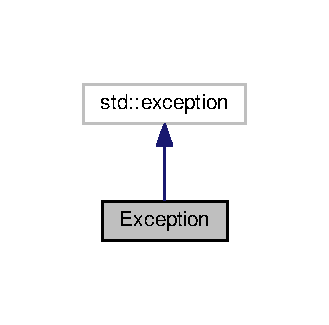
\includegraphics[width=158pt]{classException__inherit__graph}
\end{center}
\end{figure}


Diagrama de colaboración para Exception\+:
\nopagebreak
\begin{figure}[H]
\begin{center}
\leavevmode
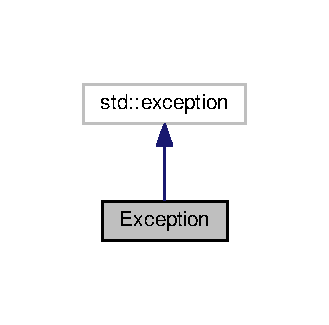
\includegraphics[width=158pt]{classException__coll__graph}
\end{center}
\end{figure}
\subsection*{Métodos públicos}
\begin{DoxyCompactItemize}
\item 
\hyperlink{classException_ac541ead5c20548813d7dea73c28c7fab}{Exception} (const char $\ast$message)
\begin{DoxyCompactList}\small\item\em Constructor (C strings). \end{DoxyCompactList}\item 
\hyperlink{classException_a472b7904dadf1047ba48c23741888456}{Exception} (const std\+::string \&message)
\begin{DoxyCompactList}\small\item\em Constructor (C++ S\+TL strings). \end{DoxyCompactList}\item 
virtual \hyperlink{classException_ad1ba411de295ef2eeb02ba26284a829a}{$\sim$\+Exception} ()  throw ()
\begin{DoxyCompactList}\small\item\em Destructor. \end{DoxyCompactList}\item 
virtual const char $\ast$ \hyperlink{classException_a78154a31544a609cbd226d32574f52cd}{what} () const   throw ()
\begin{DoxyCompactList}\small\item\em Returns a pointer to the (constant) error description. \end{DoxyCompactList}\end{DoxyCompactItemize}
\subsection*{Atributos protegidos}
\begin{DoxyCompactItemize}
\item 
std\+::string \hyperlink{classException_a5d59cc46086c61391ed26773ce861780}{msg\+\_\+}\hypertarget{classException_a5d59cc46086c61391ed26773ce861780}{}\label{classException_a5d59cc46086c61391ed26773ce861780}

\begin{DoxyCompactList}\small\item\em Error message. \end{DoxyCompactList}\end{DoxyCompactItemize}


\subsection{Documentación del constructor y destructor}
\index{Exception@{Exception}!Exception@{Exception}}
\index{Exception@{Exception}!Exception@{Exception}}
\subsubsection[{\texorpdfstring{Exception(const char $\ast$message)}{Exception(const char *message)}}]{\setlength{\rightskip}{0pt plus 5cm}Exception\+::\+Exception (
\begin{DoxyParamCaption}
\item[{const char $\ast$}]{message}
\end{DoxyParamCaption}
)\hspace{0.3cm}{\ttfamily [inline]}, {\ttfamily [explicit]}}\hypertarget{classException_ac541ead5c20548813d7dea73c28c7fab}{}\label{classException_ac541ead5c20548813d7dea73c28c7fab}


Constructor (C strings). 


\begin{DoxyParams}{Parámetros}
{\em message} & C-\/style string error message. The string contents are copied upon construction. Hence, responsibility for deleting the char$\ast$ lies with the caller. \\
\hline
\end{DoxyParams}
\index{Exception@{Exception}!Exception@{Exception}}
\index{Exception@{Exception}!Exception@{Exception}}
\subsubsection[{\texorpdfstring{Exception(const std\+::string \&message)}{Exception(const std::string &message)}}]{\setlength{\rightskip}{0pt plus 5cm}Exception\+::\+Exception (
\begin{DoxyParamCaption}
\item[{const std\+::string \&}]{message}
\end{DoxyParamCaption}
)\hspace{0.3cm}{\ttfamily [inline]}, {\ttfamily [explicit]}}\hypertarget{classException_a472b7904dadf1047ba48c23741888456}{}\label{classException_a472b7904dadf1047ba48c23741888456}


Constructor (C++ S\+TL strings). 


\begin{DoxyParams}{Parámetros}
{\em message} & The error message. \\
\hline
\end{DoxyParams}
\index{Exception@{Exception}!````~Exception@{$\sim$\+Exception}}
\index{````~Exception@{$\sim$\+Exception}!Exception@{Exception}}
\subsubsection[{\texorpdfstring{$\sim$\+Exception()}{~Exception()}}]{\setlength{\rightskip}{0pt plus 5cm}virtual Exception\+::$\sim$\+Exception (
\begin{DoxyParamCaption}
{}
\end{DoxyParamCaption}
) throw  ) \hspace{0.3cm}{\ttfamily [inline]}, {\ttfamily [virtual]}}\hypertarget{classException_ad1ba411de295ef2eeb02ba26284a829a}{}\label{classException_ad1ba411de295ef2eeb02ba26284a829a}


Destructor. 

Virtual to allow for subclassing. 

\subsection{Documentación de las funciones miembro}
\index{Exception@{Exception}!what@{what}}
\index{what@{what}!Exception@{Exception}}
\subsubsection[{\texorpdfstring{what() const }{what() const }}]{\setlength{\rightskip}{0pt plus 5cm}virtual const char$\ast$ Exception\+::what (
\begin{DoxyParamCaption}
{}
\end{DoxyParamCaption}
) const throw  ) \hspace{0.3cm}{\ttfamily [inline]}, {\ttfamily [virtual]}}\hypertarget{classException_a78154a31544a609cbd226d32574f52cd}{}\label{classException_a78154a31544a609cbd226d32574f52cd}


Returns a pointer to the (constant) error description. 

\begin{DoxyReturn}{Devuelve}
A pointer to a const char$\ast$. The underlying memory is in posession of the \hyperlink{classException}{Exception} object. Callers must not attempt to free the memory. 
\end{DoxyReturn}


La documentación para esta clase fue generada a partir del siguiente fichero\+:\begin{DoxyCompactItemize}
\item 
exception.\+h\end{DoxyCompactItemize}

\hypertarget{classmethods_1_1Liebmann}{}\section{Referencia de la plantilla de la Clase methods\+:\+:Liebmann$<$ T $>$}
\label{classmethods_1_1Liebmann}\index{methods\+::\+Liebmann$<$ T $>$@{methods\+::\+Liebmann$<$ T $>$}}
\subsection*{Métodos públicos}
\begin{DoxyCompactItemize}
\item 
\hyperlink{classmethods_1_1Liebmann_a7a095aca7a7556f4eec22c2c3528f436}{Liebmann} ()\hypertarget{classmethods_1_1Liebmann_a7a095aca7a7556f4eec22c2c3528f436}{}\label{classmethods_1_1Liebmann_a7a095aca7a7556f4eec22c2c3528f436}

\begin{DoxyCompactList}\small\item\em Constructor. \end{DoxyCompactList}\item 
\hyperlink{classmethods_1_1Liebmann_a2f2d48f06aeb92dcbcb0e73774ffb200}{$\sim$\+Liebmann} ()\hypertarget{classmethods_1_1Liebmann_a2f2d48f06aeb92dcbcb0e73774ffb200}{}\label{classmethods_1_1Liebmann_a2f2d48f06aeb92dcbcb0e73774ffb200}

\begin{DoxyCompactList}\small\item\em Destructor. \end{DoxyCompactList}\item 
const char $\ast$ {\bfseries convert\+To\+String} (std\+::vector$<$ T $>$ V)\hypertarget{classmethods_1_1Liebmann_aa08c0ff64a59ca72fbb3d1d4d0e690bc}{}\label{classmethods_1_1Liebmann_aa08c0ff64a59ca72fbb3d1d4d0e690bc}

\item 
void \hyperlink{classmethods_1_1Liebmann_a883dbcefab3121f882abefd7740fe057}{liebmann} (short int n, short int m, T bottom, T top, T left, T right, std\+::vector$<$ T $>$ \&solution, T umbral)
\begin{DoxyCompactList}\small\item\em Este es el metodo utilizado para generar la matriz de solucion del metodo de liebman paralelizado. \end{DoxyCompactList}\item 
void \hyperlink{classmethods_1_1Liebmann_aa89b8c2b82ca711b58fa318b1279ace0}{pliebmann} (short int n, short int m, T bottom, T top, T left, T right, std\+::vector$<$ T $>$ \&solution)
\begin{DoxyCompactList}\small\item\em Este es el metodo utilizado para generar la matriz de solucion del metodo de liebmann paralelizado. \end{DoxyCompactList}\item 
void \hyperlink{classmethods_1_1Liebmann_a21db65627b967d86d1cd5fd0c60e9cfb}{heatX} (int n, int m, std\+::vector$<$ T $>$ \&qx, std\+::vector$<$ T $>$ V)
\begin{DoxyCompactList}\small\item\em Este es el metodo utilizado para generar el vector qx, que representa la componente x del flujo del calor. \end{DoxyCompactList}\item 
void \hyperlink{classmethods_1_1Liebmann_ade173b06f3fb835d5bab07c9307052db}{heatY} (int n, int m, std\+::vector$<$ T $>$ \&qy, std\+::vector$<$ T $>$ V)
\begin{DoxyCompactList}\small\item\em Este es el metodo utilizado para generar el vector qy, que representa la componente y del flujo del calor. \end{DoxyCompactList}\end{DoxyCompactItemize}


\subsection{Documentación de las funciones miembro}
\index{methods\+::\+Liebmann@{methods\+::\+Liebmann}!heatX@{heatX}}
\index{heatX@{heatX}!methods\+::\+Liebmann@{methods\+::\+Liebmann}}
\subsubsection[{\texorpdfstring{heat\+X(int n, int m, std\+::vector$<$ T $>$ \&qx, std\+::vector$<$ T $>$ V)}{heatX(int n, int m, std::vector< T > &qx, std::vector< T > V)}}]{\setlength{\rightskip}{0pt plus 5cm}template$<$typename T $>$ void {\bf methods\+::\+Liebmann}$<$ T $>$\+::heatX (
\begin{DoxyParamCaption}
\item[{int}]{n, }
\item[{int}]{m, }
\item[{std\+::vector$<$ T $>$ \&}]{qx, }
\item[{std\+::vector$<$ T $>$}]{V}
\end{DoxyParamCaption}
)}\hypertarget{classmethods_1_1Liebmann_a21db65627b967d86d1cd5fd0c60e9cfb}{}\label{classmethods_1_1Liebmann_a21db65627b967d86d1cd5fd0c60e9cfb}


Este es el metodo utilizado para generar el vector qx, que representa la componente x del flujo del calor. 


\begin{DoxyParams}{Parámetros}
{\em n} & indica el numero de filas que va a tener la matriz \\
\hline
{\em m} & indica el numero de columnas que va a tener la matriz \\
\hline
{\em qx} & vector representante de la componente x del flujo calorifico \\
\hline
{\em top} & indica la cantidad de calor que se va a aplicar al lado de arriba de la placa (el valor es constante por todo el lado), si el valor que se indica es 0, se asume que ese borde esta aislado \\
\hline
{\em V} & representa el vector soluci\mbox{[}on del metodo de liebmann \\
\hline
\end{DoxyParams}
\index{methods\+::\+Liebmann@{methods\+::\+Liebmann}!heatY@{heatY}}
\index{heatY@{heatY}!methods\+::\+Liebmann@{methods\+::\+Liebmann}}
\subsubsection[{\texorpdfstring{heat\+Y(int n, int m, std\+::vector$<$ T $>$ \&qy, std\+::vector$<$ T $>$ V)}{heatY(int n, int m, std::vector< T > &qy, std::vector< T > V)}}]{\setlength{\rightskip}{0pt plus 5cm}template$<$typename T $>$ void {\bf methods\+::\+Liebmann}$<$ T $>$\+::heatY (
\begin{DoxyParamCaption}
\item[{int}]{n, }
\item[{int}]{m, }
\item[{std\+::vector$<$ T $>$ \&}]{qy, }
\item[{std\+::vector$<$ T $>$}]{V}
\end{DoxyParamCaption}
)}\hypertarget{classmethods_1_1Liebmann_ade173b06f3fb835d5bab07c9307052db}{}\label{classmethods_1_1Liebmann_ade173b06f3fb835d5bab07c9307052db}


Este es el metodo utilizado para generar el vector qy, que representa la componente y del flujo del calor. 


\begin{DoxyParams}{Parámetros}
{\em n} & indica el numero de filas que va a tener la matriz \\
\hline
{\em m} & indica el numero de columnas que va a tener la matriz \\
\hline
{\em qx} & vector representante de la componente y del flujo calorifico \\
\hline
{\em top} & indica la cantidad de calor que se va a aplicar al lado de arriba de la placa (el valor es constante por todo el lado), si el valor que se indica es 0, se asume que ese borde esta aislado \\
\hline
{\em V} & representa el vector soluci\mbox{[}on del metodo de liebmann \\
\hline
\end{DoxyParams}
\index{methods\+::\+Liebmann@{methods\+::\+Liebmann}!liebmann@{liebmann}}
\index{liebmann@{liebmann}!methods\+::\+Liebmann@{methods\+::\+Liebmann}}
\subsubsection[{\texorpdfstring{liebmann(short int n, short int m, T bottom, T top, T left, T right, std\+::vector$<$ T $>$ \&solution, T umbral)}{liebmann(short int n, short int m, T bottom, T top, T left, T right, std::vector< T > &solution, T umbral)}}]{\setlength{\rightskip}{0pt plus 5cm}template$<$typename T $>$ void {\bf methods\+::\+Liebmann}$<$ T $>$\+::liebmann (
\begin{DoxyParamCaption}
\item[{short int}]{n, }
\item[{short int}]{m, }
\item[{T}]{bottom, }
\item[{T}]{top, }
\item[{T}]{left, }
\item[{T}]{right, }
\item[{std\+::vector$<$ T $>$ \&}]{solution, }
\item[{T}]{umbral}
\end{DoxyParamCaption}
)}\hypertarget{classmethods_1_1Liebmann_a883dbcefab3121f882abefd7740fe057}{}\label{classmethods_1_1Liebmann_a883dbcefab3121f882abefd7740fe057}


Este es el metodo utilizado para generar la matriz de solucion del metodo de liebman paralelizado. 

Este es el metodo utilizado para generar la matriz de solucion del metodo de liebmann.


\begin{DoxyParams}{Parámetros}
{\em n} & indica el numero de filas que va a tener la matriz \\
\hline
{\em m} & indica el numero de columnas que va a tener la matriz \\
\hline
{\em bottom} & indica la cantidad de calor que se va a aplicar al lado mas bajo de la placa (el valor es constante por todo el lado), si el valor que se indica es 0, se asume que ese borde esta aislado \\
\hline
{\em top} & indica la cantidad de calor que se va a aplicar al lado de arriba de la placa (el valor es constante por todo el lado), si el valor que se indica es 0, se asume que ese borde esta aislado \\
\hline
{\em left} & indica la cantidad de calor que se va a aplicar al lado izquierdo de la placa (el valor es constante por todo el lado), si el valor que se indica es 0, se asume que ese borde esta aislado \\
\hline
{\em right} & indica la cantidad de calor que se va a aplicar al lado derecho de la placa (el valor es constante por todo el lado), si el valor que se indica es 0, se asume que ese borde esta aislado \\
\hline
{\em solution} & En este parametro se almacenara la solucion del metodo \\
\hline
\end{DoxyParams}
se instancia una matriz en la cual se guardara la solucion del metodo

se instancia una matriz temporal en la cual se guardara la matriz anterior del metodo, para as\mbox{[}i hacer las comparaciones y obtener el error

se llena con cero la matriz

se llena con cero la matriz

se analizan los casos de los limites Para el caso de la placa es sencillo dado el hecho de que solo se analizan los bordes

Se aplica el metodo de liebmann T\mbox{[}i\mbox{]}\mbox{[}j\mbox{]} = (1/4)( T\mbox{[}i+1\mbox{]}\mbox{[}j\mbox{]} + T\mbox{[}i-\/1\mbox{]}\mbox{[}j\mbox{]} + T\mbox{[}i\mbox{]}\mbox{[}j+1\mbox{]} + T\mbox{[}i\mbox{]}\mbox{[}j-\/1\mbox{]}) el metodo se iterera n veces

tmp\+:almacena el valor de la formula

tmp\+:almacena el valor de la formula

tmp\+:almacena el valor de la formula

tmp\+:almacena el valor de la formula

tmp\+:almacena el valor de la formula

tmp\+:almacena el valor de la formula

tmp\+:almacena el valor de la formula

Se guarda el resultado de la matriz en el vector solution\index{methods\+::\+Liebmann@{methods\+::\+Liebmann}!pliebmann@{pliebmann}}
\index{pliebmann@{pliebmann}!methods\+::\+Liebmann@{methods\+::\+Liebmann}}
\subsubsection[{\texorpdfstring{pliebmann(short int n, short int m, T bottom, T top, T left, T right, std\+::vector$<$ T $>$ \&solution)}{pliebmann(short int n, short int m, T bottom, T top, T left, T right, std::vector< T > &solution)}}]{\setlength{\rightskip}{0pt plus 5cm}template$<$typename T $>$ void {\bf methods\+::\+Liebmann}$<$ T $>$\+::pliebmann (
\begin{DoxyParamCaption}
\item[{short int}]{n, }
\item[{short int}]{m, }
\item[{T}]{bottom, }
\item[{T}]{top, }
\item[{T}]{left, }
\item[{T}]{right, }
\item[{std\+::vector$<$ T $>$ \&}]{solution}
\end{DoxyParamCaption}
)}\hypertarget{classmethods_1_1Liebmann_aa89b8c2b82ca711b58fa318b1279ace0}{}\label{classmethods_1_1Liebmann_aa89b8c2b82ca711b58fa318b1279ace0}


Este es el metodo utilizado para generar la matriz de solucion del metodo de liebmann paralelizado. 

Este es el metodo utilizado para generar la matriz de solucion del metodo de leabman paralelizado.


\begin{DoxyParams}{Parámetros}
{\em n} & indica el numero de filas que va a tener la matriz \\
\hline
{\em m} & indica el numero de columnas que va a tener la matriz \\
\hline
{\em bottom} & indica la cantidad de calor que se va a aplicar al lado mas bajo de la placa (el valor es constante por todo el lado), si el valor que se indica es 0, se asume que ese borde esta aislado \\
\hline
{\em top} & indica la cantidad de calor que se va a aplicar al lado de arriba de la placa (el valor es constante por todo el lado), si el valor que se indica es 0, se asume que ese borde esta aislado \\
\hline
{\em left} & indica la cantidad de calor que se va a aplicar al lado izquierdo de la placa (el valor es constante por todo el lado), si el valor que se indica es 0, se asume que ese borde esta aislado \\
\hline
{\em right} & indica la cantidad de calor que se va a aplicar al lado derecho de la placa (el valor es constante por todo el lado), si el valor que se indica es 0, se asume que ese borde esta aislado \\
\hline
{\em solution} & En este parametro se almacenara la solucion del metodo \\
\hline
\end{DoxyParams}
se instancia una matriz en la cual se guardara la solucion del metodo

se llena con cero la matriz

se analizan los casos de los limites Para el caso de la placa es sencillo dado el hecho de que solo se analizan los bordes

Se aplica el metodo de liebmann T\mbox{[}i\mbox{]}\mbox{[}j\mbox{]} = (1/4)( T\mbox{[}i+1\mbox{]}\mbox{[}j\mbox{]} + T\mbox{[}i-\/1\mbox{]}\mbox{[}j\mbox{]} + T\mbox{[}i\mbox{]}\mbox{[}j+1\mbox{]} + T\mbox{[}i\mbox{]}\mbox{[}j-\/1\mbox{]}) el metodo se iterera n veces

tmp\+: almacena el valor de la formula del metodo de liebmann

Se guarda el resultado de la matriz en el vector solution

La documentación para esta clase fue generada a partir del siguiente fichero\+:\begin{DoxyCompactItemize}
\item 
methods.\+h\end{DoxyCompactItemize}

\hypertarget{classanpi_1_1Matrix}{}\section{Referencia de la plantilla de la Clase anpi\+:\+:Matrix$<$ T $>$}
\label{classanpi_1_1Matrix}\index{anpi\+::\+Matrix$<$ T $>$@{anpi\+::\+Matrix$<$ T $>$}}


Row-\/major simple matrix class.  




{\ttfamily \#include $<$matrix.\+h$>$}

\subsection*{Métodos públicos}
\begin{DoxyCompactItemize}
\item 
\hyperlink{classanpi_1_1Matrix_a378f41ca6eba448d5aabbbbafc9110cf}{Matrix} ()\hypertarget{classanpi_1_1Matrix_a378f41ca6eba448d5aabbbbafc9110cf}{}\label{classanpi_1_1Matrix_a378f41ca6eba448d5aabbbbafc9110cf}

\begin{DoxyCompactList}\small\item\em Construct an empty matrix. \end{DoxyCompactList}\item 
\hyperlink{classanpi_1_1Matrix_a7e948c79bd875197a3850e03efc8bd5f}{Matrix} (const size\+\_\+t \hyperlink{classanpi_1_1Matrix_a4b786272497d9f67f120a226c1bfcff4}{rows}, const size\+\_\+t \hyperlink{classanpi_1_1Matrix_a5bd9f2fe255fe0390bfe880877222b2a}{cols}, const T init\+Val=T())\hypertarget{classanpi_1_1Matrix_a7e948c79bd875197a3850e03efc8bd5f}{}\label{classanpi_1_1Matrix_a7e948c79bd875197a3850e03efc8bd5f}

\begin{DoxyCompactList}\small\item\em Construct a matrix rows x cols and initialize all elements with the given value. \end{DoxyCompactList}\item 
\hyperlink{classanpi_1_1Matrix_a3c37c93a58cbb831863ad3ad9dc73af6}{Matrix} (const size\+\_\+t \hyperlink{classanpi_1_1Matrix_a4b786272497d9f67f120a226c1bfcff4}{rows}, const size\+\_\+t \hyperlink{classanpi_1_1Matrix_a5bd9f2fe255fe0390bfe880877222b2a}{cols}, const T $\ast$const init\+Mem)\hypertarget{classanpi_1_1Matrix_a3c37c93a58cbb831863ad3ad9dc73af6}{}\label{classanpi_1_1Matrix_a3c37c93a58cbb831863ad3ad9dc73af6}

\begin{DoxyCompactList}\small\item\em Construct a matrix rows x cols and initialize all elements with the memory content at the given pointer. \end{DoxyCompactList}\item 
\hyperlink{classanpi_1_1Matrix_a336997e2f4cf238db9f2fb9992144f23}{Matrix} (const \hyperlink{classanpi_1_1Matrix}{Matrix}$<$ T $>$ \&other)\hypertarget{classanpi_1_1Matrix_a336997e2f4cf238db9f2fb9992144f23}{}\label{classanpi_1_1Matrix_a336997e2f4cf238db9f2fb9992144f23}

\begin{DoxyCompactList}\small\item\em Copy constructor will do a deep copy on the given matrix. \end{DoxyCompactList}\item 
\hyperlink{classanpi_1_1Matrix_acd9cb8d3e7b77bb14d9ce6d153ac5634}{$\sim$\+Matrix} ()\hypertarget{classanpi_1_1Matrix_acd9cb8d3e7b77bb14d9ce6d153ac5634}{}\label{classanpi_1_1Matrix_acd9cb8d3e7b77bb14d9ce6d153ac5634}

\begin{DoxyCompactList}\small\item\em Release all memory. \end{DoxyCompactList}\item 
\hyperlink{classanpi_1_1Matrix}{Matrix}$<$ T $>$ \& \hyperlink{classanpi_1_1Matrix_acba9e336b083b5d6b58fe24f7942ddbe}{operator=} (const \hyperlink{classanpi_1_1Matrix}{Matrix}$<$ T $>$ \&other)\hypertarget{classanpi_1_1Matrix_acba9e336b083b5d6b58fe24f7942ddbe}{}\label{classanpi_1_1Matrix_acba9e336b083b5d6b58fe24f7942ddbe}

\begin{DoxyCompactList}\small\item\em Deep copy another matrix. \end{DoxyCompactList}\item 
\hyperlink{classanpi_1_1Matrix}{Matrix}$<$ T $>$ \& \hyperlink{classanpi_1_1Matrix_a22e9b98af1622be5bda69334c773fc13}{operator+} (const \hyperlink{classanpi_1_1Matrix}{Matrix}$<$ T $>$ \&B)\hypertarget{classanpi_1_1Matrix_a22e9b98af1622be5bda69334c773fc13}{}\label{classanpi_1_1Matrix_a22e9b98af1622be5bda69334c773fc13}

\begin{DoxyCompactList}\small\item\em Sum this matrix with another matrix. \end{DoxyCompactList}\item 
\hyperlink{classanpi_1_1Matrix}{Matrix}$<$ T $>$ \& \hyperlink{classanpi_1_1Matrix_af9f8390a794ef305a6570c7ab4e91b84}{operator-\/} (const \hyperlink{classanpi_1_1Matrix}{Matrix}$<$ T $>$ \&B)\hypertarget{classanpi_1_1Matrix_af9f8390a794ef305a6570c7ab4e91b84}{}\label{classanpi_1_1Matrix_af9f8390a794ef305a6570c7ab4e91b84}

\begin{DoxyCompactList}\small\item\em Substract this matrix with another matrix. \end{DoxyCompactList}\item 
\hyperlink{classanpi_1_1Matrix}{Matrix}$<$ T $>$ \hyperlink{classanpi_1_1Matrix_a46d50949da215dafdb2d13e3ae4c9ac3}{operator$\ast$} (const \hyperlink{classanpi_1_1Matrix}{Matrix}$<$ T $>$ \&B)\hypertarget{classanpi_1_1Matrix_a46d50949da215dafdb2d13e3ae4c9ac3}{}\label{classanpi_1_1Matrix_a46d50949da215dafdb2d13e3ae4c9ac3}

\begin{DoxyCompactList}\small\item\em Multiplies this matrix with another matrix. \end{DoxyCompactList}\item 
T $\ast$ \hyperlink{classanpi_1_1Matrix_a6bcaaad80bd2d631017472231f6d5e63}{operator\mbox{[}$\,$\mbox{]}} (const size\+\_\+t row)\hypertarget{classanpi_1_1Matrix_a6bcaaad80bd2d631017472231f6d5e63}{}\label{classanpi_1_1Matrix_a6bcaaad80bd2d631017472231f6d5e63}

\begin{DoxyCompactList}\small\item\em Return pointer to a given row. \end{DoxyCompactList}\item 
const T $\ast$ \hyperlink{classanpi_1_1Matrix_a13da6bd67304aac627c88f7213d5593c}{operator\mbox{[}$\,$\mbox{]}} (const size\+\_\+t row) const \hypertarget{classanpi_1_1Matrix_a13da6bd67304aac627c88f7213d5593c}{}\label{classanpi_1_1Matrix_a13da6bd67304aac627c88f7213d5593c}

\begin{DoxyCompactList}\small\item\em Return read-\/only pointer to a given row. \end{DoxyCompactList}\item 
T \& \hyperlink{classanpi_1_1Matrix_aefaff4b28c12084a0c268573e96cf9ca}{operator()} (const size\+\_\+t row, const size\+\_\+t col)\hypertarget{classanpi_1_1Matrix_aefaff4b28c12084a0c268573e96cf9ca}{}\label{classanpi_1_1Matrix_aefaff4b28c12084a0c268573e96cf9ca}

\begin{DoxyCompactList}\small\item\em Return reference to the element at the r row and c column. \end{DoxyCompactList}\item 
const T \& \hyperlink{classanpi_1_1Matrix_aedfd2cc5d14302bac723cafc08cc026a}{get} (const size\+\_\+t row, const size\+\_\+t col) const \hypertarget{classanpi_1_1Matrix_aedfd2cc5d14302bac723cafc08cc026a}{}\label{classanpi_1_1Matrix_aedfd2cc5d14302bac723cafc08cc026a}

\begin{DoxyCompactList}\small\item\em Return const reference to the element at the r row and c column. \end{DoxyCompactList}\item 
void \hyperlink{classanpi_1_1Matrix_a3cfc6c7134e51144233c27277577dbd1}{insert} (const size\+\_\+t row, const size\+\_\+t col, T \hyperlink{classanpi_1_1Matrix_ad620d822fefc019cef07f4c1fb1c7052}{data}) const 
\begin{DoxyCompactList}\small\item\em insert the data into the row and col space \end{DoxyCompactList}\item 
void \hyperlink{classanpi_1_1Matrix_ac3ac962e6058ef48b58e654e4ea7ed65}{allocate} (const size\+\_\+t row, const size\+\_\+t col)\hypertarget{classanpi_1_1Matrix_ac3ac962e6058ef48b58e654e4ea7ed65}{}\label{classanpi_1_1Matrix_ac3ac962e6058ef48b58e654e4ea7ed65}

\begin{DoxyCompactList}\small\item\em Allocate memory for the given number of rows and cols. \end{DoxyCompactList}\item 
void \hyperlink{classanpi_1_1Matrix_ad7b7f6f61d23ae8ccd7e3a19e82a8c63}{fill} (const T val)\hypertarget{classanpi_1_1Matrix_ad7b7f6f61d23ae8ccd7e3a19e82a8c63}{}\label{classanpi_1_1Matrix_ad7b7f6f61d23ae8ccd7e3a19e82a8c63}

\begin{DoxyCompactList}\small\item\em Fill all elements of the matrix with the given value. \end{DoxyCompactList}\item 
void \hyperlink{classanpi_1_1Matrix_a2df6d413691d4aa8d0e958eb74ee394b}{fill} (const T $\ast$mem)
\begin{DoxyCompactList}\small\item\em Fill all elements of the matrix with the given memory block. \end{DoxyCompactList}\item 
size\+\_\+t \hyperlink{classanpi_1_1Matrix_a4b786272497d9f67f120a226c1bfcff4}{rows} () const \hypertarget{classanpi_1_1Matrix_a4b786272497d9f67f120a226c1bfcff4}{}\label{classanpi_1_1Matrix_a4b786272497d9f67f120a226c1bfcff4}

\begin{DoxyCompactList}\small\item\em Number of rows. \end{DoxyCompactList}\item 
size\+\_\+t \hyperlink{classanpi_1_1Matrix_a5bd9f2fe255fe0390bfe880877222b2a}{cols} () const \hypertarget{classanpi_1_1Matrix_a5bd9f2fe255fe0390bfe880877222b2a}{}\label{classanpi_1_1Matrix_a5bd9f2fe255fe0390bfe880877222b2a}

\begin{DoxyCompactList}\small\item\em Number of columns. \end{DoxyCompactList}\item 
T $\ast$ \hyperlink{classanpi_1_1Matrix_ad620d822fefc019cef07f4c1fb1c7052}{data} ()\hypertarget{classanpi_1_1Matrix_ad620d822fefc019cef07f4c1fb1c7052}{}\label{classanpi_1_1Matrix_ad620d822fefc019cef07f4c1fb1c7052}

\begin{DoxyCompactList}\small\item\em Pointer to data block. \end{DoxyCompactList}\item 
const T $\ast$ \hyperlink{classanpi_1_1Matrix_a1f1196beed4607edc1509ede6ef26217}{data} () const \hypertarget{classanpi_1_1Matrix_a1f1196beed4607edc1509ede6ef26217}{}\label{classanpi_1_1Matrix_a1f1196beed4607edc1509ede6ef26217}

\begin{DoxyCompactList}\small\item\em Pointer to data block. \end{DoxyCompactList}\item 
const T \hyperlink{classanpi_1_1Matrix_a404201aad5948d0ccae15b65a4e2d5ad}{norm} ()\hypertarget{classanpi_1_1Matrix_a404201aad5948d0ccae15b65a4e2d5ad}{}\label{classanpi_1_1Matrix_a404201aad5948d0ccae15b65a4e2d5ad}

\begin{DoxyCompactList}\small\item\em Return the norm of the matrix. \end{DoxyCompactList}\item 
const T {\bfseries determ} ()\hypertarget{classanpi_1_1Matrix_afaf714fe0f8a2330ce080dff8a0819af}{}\label{classanpi_1_1Matrix_afaf714fe0f8a2330ce080dff8a0819af}

\end{DoxyCompactItemize}


\subsection{Descripción detallada}
\subsubsection*{template$<$typename T$>$\\*
class anpi\+::\+Matrix$<$ T $>$}

Row-\/major simple matrix class. 

\subsection{Documentación de las funciones miembro}
\index{anpi\+::\+Matrix@{anpi\+::\+Matrix}!fill@{fill}}
\index{fill@{fill}!anpi\+::\+Matrix@{anpi\+::\+Matrix}}
\subsubsection[{\texorpdfstring{fill(const T $\ast$mem)}{fill(const T *mem)}}]{\setlength{\rightskip}{0pt plus 5cm}template$<$typename T $>$ void {\bf anpi\+::\+Matrix}$<$ T $>$\+::fill (
\begin{DoxyParamCaption}
\item[{const T $\ast$}]{mem}
\end{DoxyParamCaption}
)}\hypertarget{classanpi_1_1Matrix_a2df6d413691d4aa8d0e958eb74ee394b}{}\label{classanpi_1_1Matrix_a2df6d413691d4aa8d0e958eb74ee394b}


Fill all elements of the matrix with the given memory block. 

The user must ensure that the given memory block has enough elements \index{anpi\+::\+Matrix@{anpi\+::\+Matrix}!insert@{insert}}
\index{insert@{insert}!anpi\+::\+Matrix@{anpi\+::\+Matrix}}
\subsubsection[{\texorpdfstring{insert(const size\+\_\+t row, const size\+\_\+t col, T data) const }{insert(const size_t row, const size_t col, T data) const }}]{\setlength{\rightskip}{0pt plus 5cm}template$<$typename T$>$ void {\bf anpi\+::\+Matrix}$<$ T $>$\+::insert (
\begin{DoxyParamCaption}
\item[{const size\+\_\+t}]{row, }
\item[{const size\+\_\+t}]{col, }
\item[{T}]{data}
\end{DoxyParamCaption}
) const\hspace{0.3cm}{\ttfamily [inline]}}\hypertarget{classanpi_1_1Matrix_a3cfc6c7134e51144233c27277577dbd1}{}\label{classanpi_1_1Matrix_a3cfc6c7134e51144233c27277577dbd1}


insert the data into the row and col space 


\begin{DoxyParams}{Parámetros}
{\em row} & \\
\hline
{\em col} & \\
\hline
{\em data} & \\
\hline
\end{DoxyParams}


La documentación para esta clase fue generada a partir del siguiente fichero\+:\begin{DoxyCompactItemize}
\item 
matrix.\+h\end{DoxyCompactItemize}

%--- End generated contents ---

% Index
\backmatter
\newpage
\phantomsection
\clearemptydoublepage
\addcontentsline{toc}{chapter}{Índice}
\printindex

\end{document}
